\documentclass[tikz]{standalone}
\usepackage{xcolor, amsmath, amssymb}
\usetikzlibrary{arrows.meta}
\begin{document}

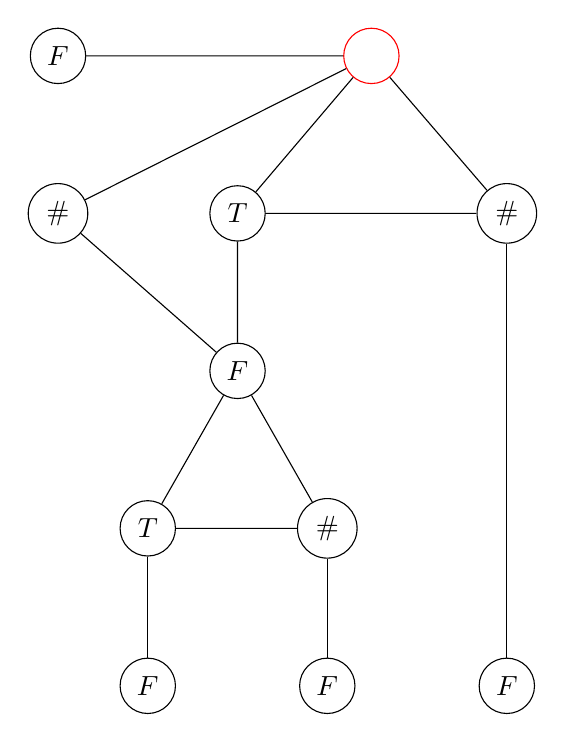
\begin{tikzpicture}[every node/.style={circle,draw},scale=2,minimum size=20pt]
\node at(-1.71,-1)(r){$\#$};
\node at(-1.71,0)(f){$F$};
\node[red] at(0.28,0)(123){};
\node at(-0.57,-1)(i12){$T$};
\node at(1.14,-1)(i3){$\#$};
\node at(-0.57,-2)(o12){$F$};
\node at(-1.14,-3)(i1){$T$};
\node at(0,-3)    (i2){$\#$};
\node at(-1.14,-4)(1){$F$};
\node at(0,-4)    (2){$F$};
\node at(1.14,-4) (3){$F$};
\draw(f)--(123)--(i12)--(i3)--(123)--(r)--(o12)--(i1)--(i2)--(o12)--(i12);
\path(1)edge(i1) (2)edge(i2) (3)edge(i3);
\end{tikzpicture}

\end{document}